\chapter{Distributed Programming (RMI)}

\section{Struttura generale dell'applicazione}
L'applicazione non è altro che il flusso operativo di un singolo nodo, che mette in mostra o recupera un oggetto attraverso l'utilizzo del registro di RMI.
\begin{figure}[H]
	\begin{center}
		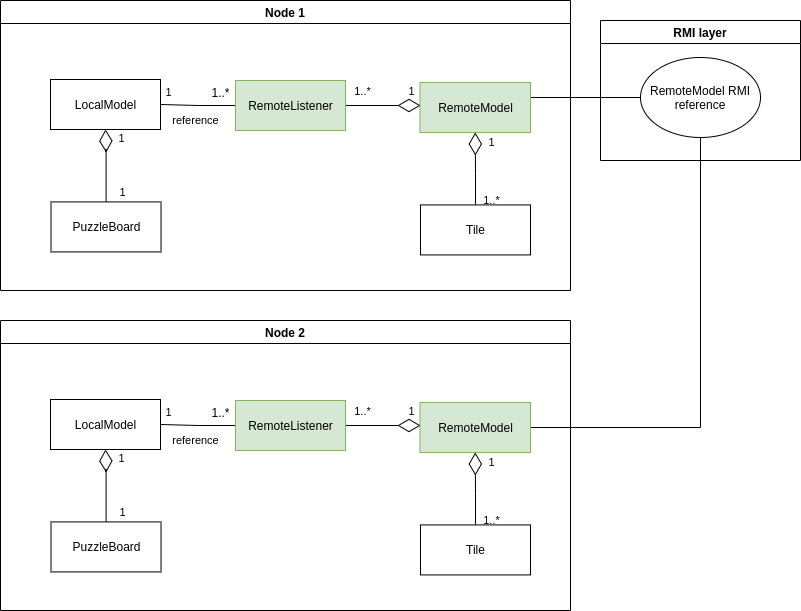
\includegraphics[width=0.8\linewidth]{img/part-2/class-rmi.png}
		\label{fig:class-rmi}
	\end{center}
	\caption{Diagramma delle classi dell'applicazione (RMI)}
\end{figure}

\subsection{Inititator e Connecting Node}
Quando un nodo vuole collegarsi, deve fare un lookup sul registro di RMI per controllare se è già presente qualche altro nodo nella rete che desidera giocare. Se non ci sono altri nodi, il nodo che ha fatto richiesta diventa l'Initiator, il quale si occuperà di creare la disposizione iniziale della scacchiera e renderla disponibile a tutti registrando un oggetto sul registro di RMI.\newline
Se ci sono altri nodi invece il riferimento all'oggetto remoto viene recuperato dal nodo attraverso il registro in modo da poterlo modificare all'occorrenza. Quando si effettua l'operazione di lookup sul registro, la label a cui è assegnata l'oggetto remoto deve essere la stessa per ogni nodo. Nel caso di questa applicazione è "model".
\subsection{LocalModel e RemoteModel}
Ogni nodo possiede due model ben distinti. Questi prendono il nome di \textit{LocalModel} e \textit{RemoteModel}.
\begin{itemize}
    \item \textbf{LocalModel}: Si tratta del Model che possiede ogni singolo nodo. Non è condiviso in nessun modo ed è completamente indipendente dal LocalModel degli altri nodi. All'interno del LocalModel c'è ad esempio la scacchiera che viene mostrata a schermo.
    \item \textbf{RemoteModel}: Si tratta dell'istanza del Model condiviso tra tutti i nodi e su cui vengono chiamati i metodi da remoto. Il nodo Initiator possiede l'istanza dell'oggetto in locale. I nodi che si connettono successivamente hanno il riferimento all'oggetto che possiede l'Initiator.
\end{itemize}
Entrambi i Model sono contenuti all'interno di un ulteriore classe di tipo Singleton che fa da wrapper e garantisce che:
\begin{itemize}
    \item Le due istanze sono le uniche nel sistema.
    \item Sia possibile richiamare le istanze in qualsiasi punto del codice.
\end{itemize}
Quando un nodo desidera modificare la disposizione della scacchiera agisce sul \textit{RemoteModel} richiamando un metodo che modifica il suo stato interno. Tutti i nodi connessi vengono quindi contattati a loro volta e viene modificato il loro LocalModel in funzione del contenuto di RemoteModel.\newline
In ogni momento il LocalModel deve contenere la stessa disposizione di Tile presente su RemoteModel.
\subsection{RemoteListener}
Quando un nodo modifica la disposizione del puzzle richiama un metodo sull'oggetto remoto che aggiorna il suo stato interno e notifica tutti i nodi, segnalando la notifica e modificando il LocalModel.\newline
È possibile grazie al pattern Observer specificare un metodo da richiamare quando lo stato interno viene modificato.\newline
Sfortunatamente l'interfaccia Observer di Java è stata deprecata a partire dalla versione 9 così come tutto il funzionamento base del pattern a causa di troppe limitazioni.\newline
Per ovviare al problema sono stati sfruttati i Listener. Un RemoteLister è un oggetto che ogni Nodo inizializza ed invia al RemoteModel quando quest'ultimo viene creato o ne viene recuperato il riferimento. Il RemoteModel quando aggiorna il suo stato interno itera su tutti i RemoteListener che possiede richiamando il metodo che verrà richiamato sul Nodo che lo aveva creato.\newline
Per poter effettuare questa operazione appena descritta è però importante ricordare che quando si passano oggetti ad un oggetto remoto questi devono soddisfare una delle due condizioni:
\begin{itemize}
    \item Implementare \textit{Serializable}. Gli oggetti che vengono passati come argomento per gli oggetti remoti vengono serializzati per poter essere inoltrati.
    \item Implementare \textit{Remote} (Interfaccia di RMI). Gli oggetti che vengono passati come argomento in questo caso non vengono serializzati. L'oggetto Remoto riceverà un riferimento dell'oggetto locale.
\end{itemize}
Se il \textit{RemoteListener} implementasse l'interfaccia \textit{Serializable}, nel momento in cui l'oggetto remoto richiamerebbe un suo metodo, questo non verrebbe richiamato sul nodo che ha creato il Listener, in quanto il Listener passato inizialmente non è altro che una sua copia serializzata.\newline
\textit{RemoteListener} deve quindi necessariamente implementare Remote. In questo modo sull'oggetto remoto arriverà un riferimento al Listener remoto che si trova sul nodo. Quando un suo metodo verrà richiamato, questo verrà eseguito sul nodo corrispondente.
\begin{minted}{java}
/**
 * Notice how this interface extends the Remote Interface.
 * This is needed as the listener will not get serialized when sent as a message,
 * it will be passed by reference allowing method calls from remote.
 */
public interface RemoteListener extends Remote {

    void onStateChange(List<Tile> newTileList) throws RemoteException;

    void onListenerAdd(Set<RemoteListener> remoteListeners) throws RemoteException;

}
\end{minted}
In particolare quando il metodo \textit{onStateChange()} viene richiamato, il nodo aggiorna il puzzle (LocalModel) con la nuova disposizione.
\section{Gestione dei fallimenti}
\subsection{Crash di un Nodo}
Se un nodo decide di andarsene o viene chiuso inaspettatamente (e non si trattava dell'Initiator), non ci sono problemi dal punto di vista di tutti gli altri nodi. Tuttavia il rispettivo RemoteListener rimane referenziato all'interno dell'oggetto remoto, e verrà sicuramente chiamato il metodo \textit{onStateChange()} su un oggetto remoto che ormai non esiste più quando qualcuno cambierà la disposizione del Puzzle.\newline
Questo però non è un problema, in quanto chiamare un metodo su un oggetto remoto che non esiste fa scaturire una \textit{RemoteException} che è possibile catturare.\newline
Quando si itera sulla collezione di Listener che si trovano sull'oggetto remoto e si cattura un eccezione di quel tipo è sufficiente rimuovere il relativo RemoteListener dalla collezione. In questo modo l'oggetto viene completamente deferenziato.
\begin{warn}[ATTENZIONE:]
    È importante non rimuovere l'oggetto direttamente mentre si itera sulla collezione se si usa un foreach, in quanto questo scaturirebbe una \textit{ConcurrentOperationException}.
\end{warn}
\subsection{Crash del Nodo Initiator}
Se è il Nodo Initiator ad andarsene mentre altri nodi stanno giocando sorge però un problema. L'istanza del RemoteModel si trovava sul Nodo che è appena andato in Crash, l'oggetto è stato distrutto, ma gli altri nodi ne hanno ancora la reference. Se un qualsiasi nodo prova a muovere delle caselle otterrà un'eccezione nel momento in cui proverà a chiamare il metodo remoto.\newline
È possibile in questo caso ristabilire la situazione.
\subsubsection{Ripristino del RemoteModel (caso ad alto livello)}
Ogni nodo possiede la situazione del puzzle anche se il nodo Initiator se n'è andato. Tramite il registro di RMI è possibile effettuare il rebind di un nuovo oggetto RemoteModel costruito da un nodo che prenderà le veci di Initiator.\newline
Quindi, in un esempio in cui tre nodi \textit{A}, \textit{B} e \textit{C} stanno giocando:
\begin{enumerate}
    \item Il Nodo Initiator \textit{A} se ne va (a causa di crash o di sua spontanea volontà). Rimangono solo \textit{B} e \textit{C}, ma nessuno si è ancora accorto che \textit{A} è sparito.
    \item Un altro nodo \textit{B} prova ad accedere all'oggetto remoto, ma ottiene una spiacevole eccezione di tipo \textit{RemoteException}.
    \item Il nodo si rende quindi conto che non è più disponibile un oggetto remoto e si occupa di ricrearlo e di effettuare l'operazione di Rebind. Inoltre finisce la sua mossa.
    \item Ora \textit{C} si accorge che qualche nodo ha effettuato una mossa, dato che il suo LocalModel è stato aggiornato. Dal suo punto di vista \textit{A} non se n'è andato e \textit{B} non è diventato un nodo più speciale di prima.
    \item Se \textit{C} prova ad effettuare una mossa riuscirà perfettamente nel suo intento, dato che la Reference al suo oggetto è stata perfettamente ricreata da \textit{B}.
\end{enumerate}

\noindent L'esempio precedente non tiene conto di una situazione più pessimistica:

\begin{enumerate}
    \item Il Nodo Initiator \textit{A} se ne va (a causa di crash o di sua spontanea volontà). Rimangono solo \textit{B} e \textit{C}, ma nessuno si è ancora accorto che \textit{A} è sparito.
    \item Un altro nodo \textit{B} prova ad accedere all'oggetto remoto, ma ottiene una spiacevole eccezione di tipo \textit{RemoteException}.
    \item Il nodo si rende quindi conto che non è più disponibile un oggetto remoto e si occupa di ricrearlo e di effettuare l'operazione di Rebind. Inoltre finisce la sua mossa.
    \item Anche \textit{C}, esattamente nello stesso momento effettua una mossa, e si rende conto che non esiste più un riferimento al RemoteModel, quindi anche lui ne crea uno ed effettua il Rebind.
    \item L'oggetto è stato ricreato da entrambi i nodi, ma sicuramente uno dei due nodi sovrascrive la mossa dell'altro.
\end{enumerate}

\noindent La successione di eventi appena descritta non rappresenta però un problema. Indipendentemente dal nodo che riesce a ricreare il RemoteModel, il riferimento a tale oggetto non cambierà, e la situazione in ambo i LocalModel sarà la medesima grazie ai Listener che notificheranno a tutti i nodi gli aggiornamenti allo stato, che avvengono all'interno di un metodo synchronized. Queste casistiche si possono applicare in modo generalizzato ad un sistema con \textit{n} nodi anziché 2.

\subsubsection{Ripristino del RemoteModel (Problema dei Listener)}
Non è un problema ripristinare l'istanza di un RemoteModel a partire dal LocalModel di un altro nodo. Lo stato del puzzle viene ricreato senza problemi nell'oggetto remoto. Il problema è che RemoteModel non è composto solamente dallo stato del puzzle, ma anche dai vari Listener che vengono registrati quando un nodo acquisisce il riferimento all'oggetto RemoteModel dal registro.\newline
Nessun nodo ha interesse a mantenere anche questi riferimenti ad oggetto nel proprio LocalModel. Secondo l'architettura proposta ogni nodo dovrebbe essere legato solo al proprio Listener e non dovrebbe possedere i Listener altrui.\newline
Tuttavia, se i singoli nodi non salvassero a loro volta i riferimenti a questi oggetti non sarebbe possibile recuperare l'esatto stato del RemoteModel, e le modifiche al puzzle non verrebbero inviate agli altri peer.\newline

\noindent La soluzione è quindi aggiungere un metodo al Listener che notifica quando un nuovo Listener viene aggiunto al RemoteModel. Questo metodo si occupa di rimandare ad ogni peer la collezione aggiornata con tutti i riferimenti ai Listener, in modo da poterli salvare all'interno del LocalModel.\newline
Ora qualsiasi peer potrà ricreare la stessa identica istanza di RemoteModel a partire dal proprio LocalModel.

\subsubsection{Arrivo di un nodo quando RemoteModel non referenziato}
Può capitare che un nodo voglia partecipare alla risoluzione del puzzle ma effettui l'operazione di join in un momento spiacevole.\newline
Il problema viene illustrato con il seguente esempio, sfruttando sempre tre peer i cui nomi sono \textit{A}, \textit{B} e \textit{C}:
\begin{enumerate}
    \item Il nodo \textit{A} crea il puzzle e lo rende disponibile ad altri peer. \textit{A} è quindi l'initiator.
    \item Il nodo \textit{B} effettua l'operazione di join, recupera quindi lo stato remoto del puzzle e lo copia in locale.
    \item Il Nodo Initiator \textit{A} se ne va (a causa di crash o di sua spontanea volontà). Rimane solo \textit{B}.
    \item Un altro nodo \textit{C} effettua l'operazione di join, prova quindi a recuperare lo stato remoto.
\end{enumerate}
\begin{warn}[PROBLEMA:]
    \textit{B} non ha ancora eseguito neanche una mossa, quindi non sa che \textit{A} se n'è andato. L'oggetto RemoteModel è registrato ma non referenziato, e \textit{C} non riesce ad accedervi per copiarlo in locale.
\end{warn}

\noindent Il problema si risolve effettuando polling durante l'operazione di connessione. Qualora l'accesso all'oggetto remoto andasse a buon fine non ci sarebbero problemi.
Se invece provando ad accedere a RemoteModel si ottiene una \textit{ServerException} allora si ritenta la connessione finché l'istanza non sarà effettivamente accedibile. Il tentativo di riconnessione avviene di base ogni 500ms.
